% -*- LaTeX -*-
% -*- coding: utf-8 -*-
%
% ~~~~~~~~~~~~~~~~~~~~~~~~~~~~~~~~~~~~~~~~~~~~~~~~~~~~~~~~~~~~~~~~~~~~~~~~~~~~~~
%
%                             michael a.g. aïvázis
%                      california institute of technology
%                      (c) 1998-2010  all rights reserved
%
% ~~~~~~~~~~~~~~~~~~~~~~~~~~~~~~~~~~~~~~~~~~~~~~~~~~~~~~~~~~~~~~~~~~~~~~~~~~~~~~
%

\lecture{Geometrical}{20100301}

% --------------------------------------
% contact detection
\begin{frame}[fragile]
%
  \frametitle{A more careful look at contact detection}
%
  \begin{itemize}
%
  \item consider a collection of tetrahedral meshes that model bodies in relative motion with
    triangular meshes as boundaries
%
  \item during the simulation, the bodies may come in contact
    \begin{itemize}
    \item with each other or themselves
    \item {\em contact events} consist of intersections among nodes, edges or faces
    \item unless the mechanics is informed of the contact events, the objects will
      inter-penetrate
    \item contact {\em detection} involves isolating the pairs of topological entities from
      each boundary that have intersected, whereas contact {\em resolution} refers to the
      calculation of appropriate restoring forces on the bodies
    \end{itemize}
%
  \item the typical simulation update step proceeds along the following lines
    \begin{enumerate}
    \item define the contact surfaces at time $t$
    \item predict the location of the nodes at a later time $t+\Delta t$ by integrating the
      equations of motion
    \item search for potential contact events among nodes, edges and faces to identify the
      contact candidates \label{item:contact-crude}
    \item perform a detailed search to isolate the entities that come in actual
      contact \label{item:contact-detailed}
    \item correct the future location of the nodes by applying forces that tend to remove the
      overlap
    \end{enumerate}
%
  \end{itemize}
%
\end{frame}

% --------------------------------------
% contact search
\begin{frame}[fragile]
%
  \frametitle{Contact search}
%
  \begin{itemize}
%
  \item the contact candidate identification in Step~\ref{item:contact-crude} and
    Step~\ref{item:contact-detailed} above have the potential to dominate the calculation
    \begin{itemize}
    \item given a candidate pair, the intersection logic involves very expensive geometrical
      calculations
    \item na\"ive algorithms are \order{n^{2}} in the number of topological entities on the
      boundary, prohibitively expensive even for moderate size calculations
    \end{itemize}
%
  \item hence, a more sensible strategy is to break the contact search up into two separate steps
    \begin{itemize}
    \item find a relatively fast algorithm to narrow down the candidates to a small number
    \item perform the detailed calculations on the reduced set
    \end{itemize}
%
  \item the search in Step~\ref{item:contact-crude} requires a specialized data structure that
    can encode the locations of the mesh nodes to support fast queries
    \begin{itemize}
    \item build a bounding box that contains the initial and final position of a given surface
      element, perhaps in some reduced form 
    \item enlarge this box to account for the motion of the nodes
    \end{itemize}
%
  \end{itemize}
%
\end{frame}



% --------------------------------------
% volume-based contact detection
\begin{frame}[fragile]
%
  \frametitle{Volume based contact detection}
%
  \begin{itemize}
%
  \item volume based approaches replace the elements on the boundary with equivalent spheres
  \item a variety of geometrical criteria can be used: 
    \begin{itemize}
      \item equivalent volume
      \item diameter determined by the longest edge
    \end{itemize}
% 
  \item contact detection can take place very efficiently using ORQ algorithms
  \item simple spring models resolve the contact forces
    \begin{itemize}
    \item based on simple potentials that take into account the sphere inter-penetration
    \end{itemize}
%
  \end{itemize}
%
  \begin{figure}
    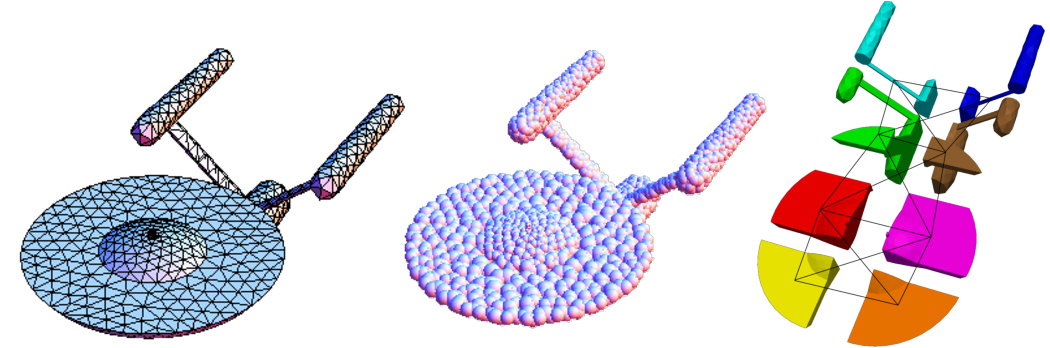
\includegraphics[scale=0.5]{figures/mesh-volumecontact.pdf}
  \end{figure}
%
\end{frame}

% --------------------------------------
% overview of contact
\begin{frame}[fragile]
%
  \frametitle{Who knows?}
%
  \begin{itemize}
%
  \item
%
  \end{itemize}
%
\end{frame}


% end of file 
